\section{Desarrollo}
% Metodologia / Desarrollo
Partiendo del que el total de combinacioneses posibles es $18! = 6,402,373,705,728,000$ sabemos que no es posible evaluar todas las combinacioneses
sin embargo en este caso debemos tomar en cuenta que existen restricciones en las rutas, por lo que el numero de combinacioneses posibles se reduce, 
pero aun asi sigue siendo un numero muy grande, por lo que se opta por usar un algoritmo genetico.

\subsection{Codificación}
En este caso, generaremos cada cromosoma como una permutación de las ciudades, representando una ruta posible para el vendedor viajero.
Cada gen en el cromosoma corresponde a una ciudad, y la secuencia de genes determina el orden en que se visitan las ciudades. Sin embargo,
debido a las restricciones en las rutas, algunas permutaciones pueden ser inválidas las cuales podemos listar en una ``tabla taboo''
\[
[8, 12, 17, 4, 10, 9, 2, 16, 1, 14, 5, 6, 7, 15, 3, 11, 13, 18]
\]
\subsection{Restricciones de Rutas Tabú}

Las siguientes combinaciones representan pares de ciudades cuya conexión directa está prohibida en el recorrido (rutas tabú):

\begin{multicols}{3}
\begin{itemize}\label{Lista taboo}
    \item (1, 7), (1, 8), (1, 17), (1, 18)
    \item (2, 6), (2, 7), (2, 8), (2, 17), (2, 18)
    \item (3, 9), (3, 10), (3, 16)
    \item (4, 7), (4, 8), (4, 11)
    \item (5, 15)
    \item (6, 2), (6, 9), (6, 14), (6, 15)
    \item (7, 1), (7, 2), (7, 4), (7, 14), (7, 18)
    \item (8, 1), (8, 2), (8, 4), (8, 14), (8, 15), (8, 16), (8, 18)
    \item (9, 3), (9, 6), (9, 15), (9, 18)
    \item (10, 3), (10, 17), (10, 18)
    \item (11, 4), (11, 16), (11, 17), (11, 18)
    \item (14, 6), (14, 7), (14, 8)
    \item (15, 5), (15, 6), (15, 8), (15, 9), (15, 16), (15, 18)
    \item (16, 3), (16, 8), (16, 11), (16, 15)
    \item (17, 1), (17, 2), (17, 10), (17, 11)
    \item (18, 1), (18, 2), (18, 7), (18, 8), (18, 9), (18, 10), (18, 11), (18, 15)
\end{itemize}
\end{multicols}

\noindent
Cada par \((i, j)\) indica que la conexión entre las ciudades \(i\) y \(j\) no está permitida dentro del recorrido, y por tanto el algoritmo genético debe evitar dichas transiciones al generar nuevas rutas.

\begin{figure}[H]
    \centering
    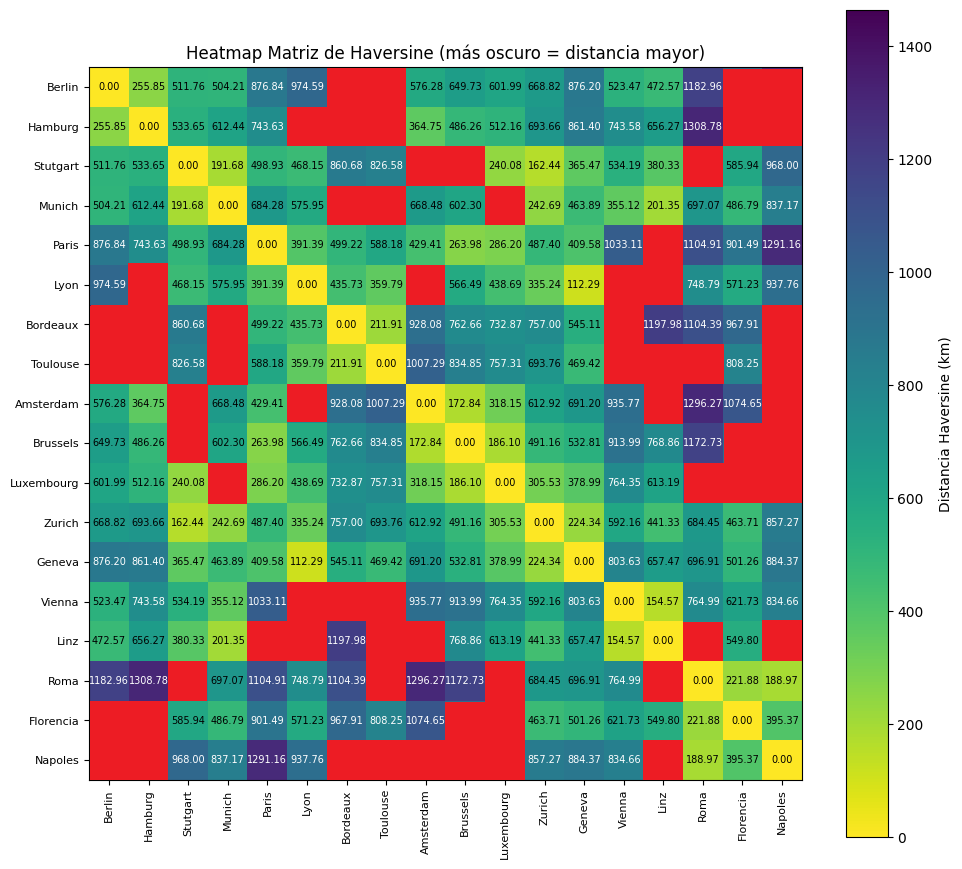
\includegraphics[width=0.85\textwidth]{rsc/img/des/taboo.png}
    \caption{Matriz de Haversine con rutas tabú marcadas en rojo}\label{fig: Matriz con restricciones}
\end{figure}

\subsection{Generar Individuo Inicial Valido}
Para generar a nuestros individuos iniciales, se crean cromosomas (rutas) de manera aleatoria, asegurando que cada ciudad se visite exactamente una vez en cada ruta.
Sin embargo, debido a las restricciones de rutas tabú, es posible que algunas rutas generadas inicialmente sean inválidas. Para manejar esto, se implementa una
función que verifica cada par $(i,j)$ en la ruta generada para generar rutas validas.

\begin{figure}[H]
    \centering
    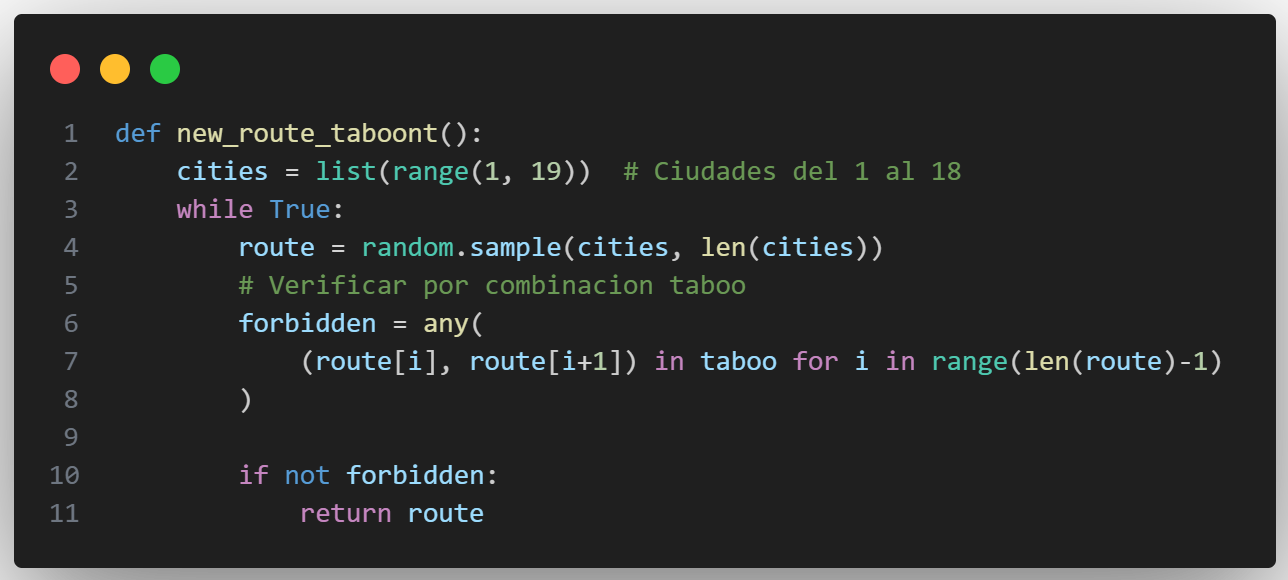
\includegraphics[width=0.65\textwidth]{rsc/img/des/funcion_taboont.png}
    \caption{Funcion generadora de un cromosoma valido}\label{fig: funcion taboont}
\end{figure}

\subsection{Evaluar Aptitud}
La función de aptitud evalúa la calidad de cada cromosoma (ruta) en la población. En este caso, la aptitud se mide por la distancia total recorrida en la ruta.
Esta se calcula sumando las distancias entre ciudades consecutivas en el cromosoma, utilizando la matriz de distancias predefinida, en este caso usaremos
la matriz de la figura~\ref{fig: Matriz con restricciones}. 

\begin{figure}[H]
    \centering
    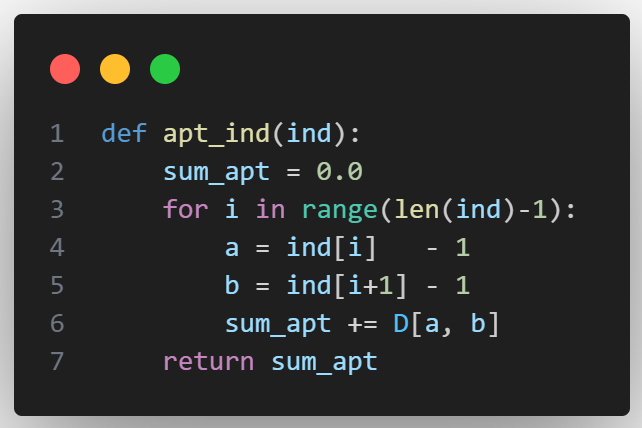
\includegraphics[width=0.75\textwidth]{rsc/img/des/funcion_apt.png}
    \caption{Funcion de aptitud}\label{fig: funcion aptitud}
\end{figure}

\subsection{Generar población}
Una vez definida la función para generar individuos válidos así como para evaluar su aptitud, se crea una población inicial
de cromosomas (rutas) utilizando la siguiente función:
\begin{figure}[H]
    \centering
    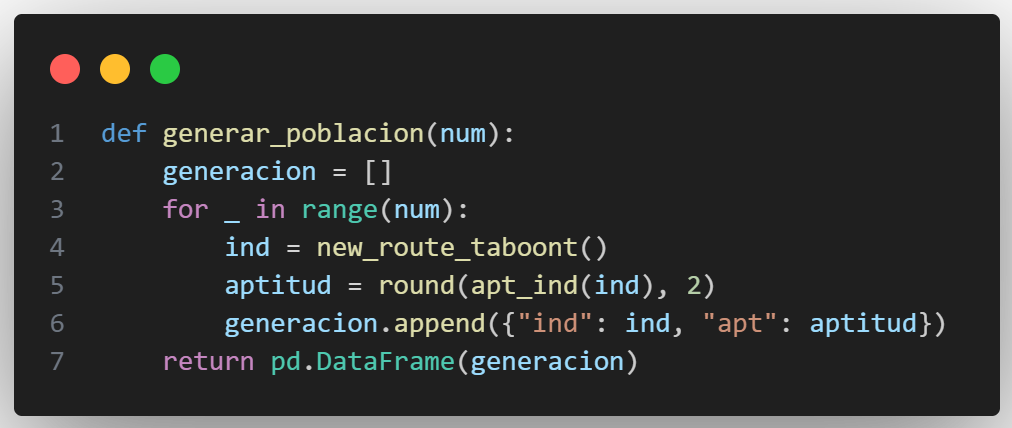
\includegraphics[width=0.75\textwidth]{rsc/img/des/funcion_gen_pob.png}
    \caption{Funcion para generar poblacion inicial}\label{fig: funcion poblacion}
\end{figure}

Con esta función, generaremos 3 conjuntos de poblaciones iniciales con tamaños de 100, 500 y 1000 individuos cada una para 
evaluar el desempeño del algoritmo genético bajo diferentes condiciones.

\subsection{Ordenamiento}
Para seleccionar los mejores individuos de la población, se implementa una función de ordenamiento basada en la aptitud de cada cromosoma.

\begin{figure}[H]
    \centering
    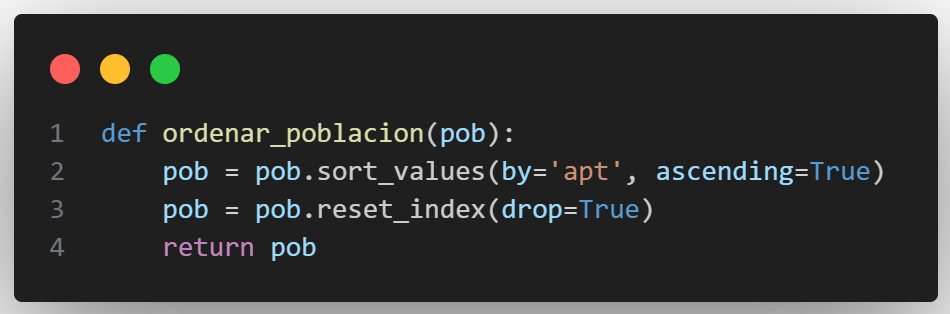
\includegraphics[width=0.75\textwidth]{rsc/img/des/ordenar.png}
    \caption{Funcion de ordenamiento de la poblacion}\label{fig: funcion ordenamiento}
\end{figure}

\subsection{Selección}
Para la selección de padres en el proceso de cruce, usaremos los metodos de torneo y ranking, para lo cual en cada generacion tomaremos la mitad 
superior de la poblacion ordenada para aplicar rank y la mitad inferior para aplicar torneo, esto con el objetivo de mantener diversidad en la 
poblacion y evitar caer en un minimo local.

\begin{figure}[H]
    \centering
    \begin{subfigure}{0.45\textwidth}
        
\includegraphics[width=1\textwidth]{rsc/img/des/rank.png}
        \caption{Funcion ranking}\label{rank}
    \end{subfigure}
    \hfill
    \begin{subfigure}{0.45\textwidth}
        
\includegraphics[width=1\textwidth]{rsc/img/des/torneo.png}
        \caption{Funcion torneo}\label{torneo}
    \end{subfigure}
    \caption{Funciones de seleccion de padres}\label{seleccion}
\end{figure}

\subsection{Cruce}

Se emplearán dos operadores de cruce: PMX (Partially Mapped Crossover) y PBX (Position-Based Crossover). 
El primero selecciona un segmento de la ruta de un padre y lo mapea en la del otro, garantizando que no existan ciudades repetidas 
mediante un proceso de correspondencia entre genes. El segundo elige posiciones aleatorias del primer padre para copiarlas directamente
al descendiente, mientras que las posiciones restantes se completan con las ciudades del segundo padre, respetando su orden relativo.

\begin{figure}[H]
    \centering
    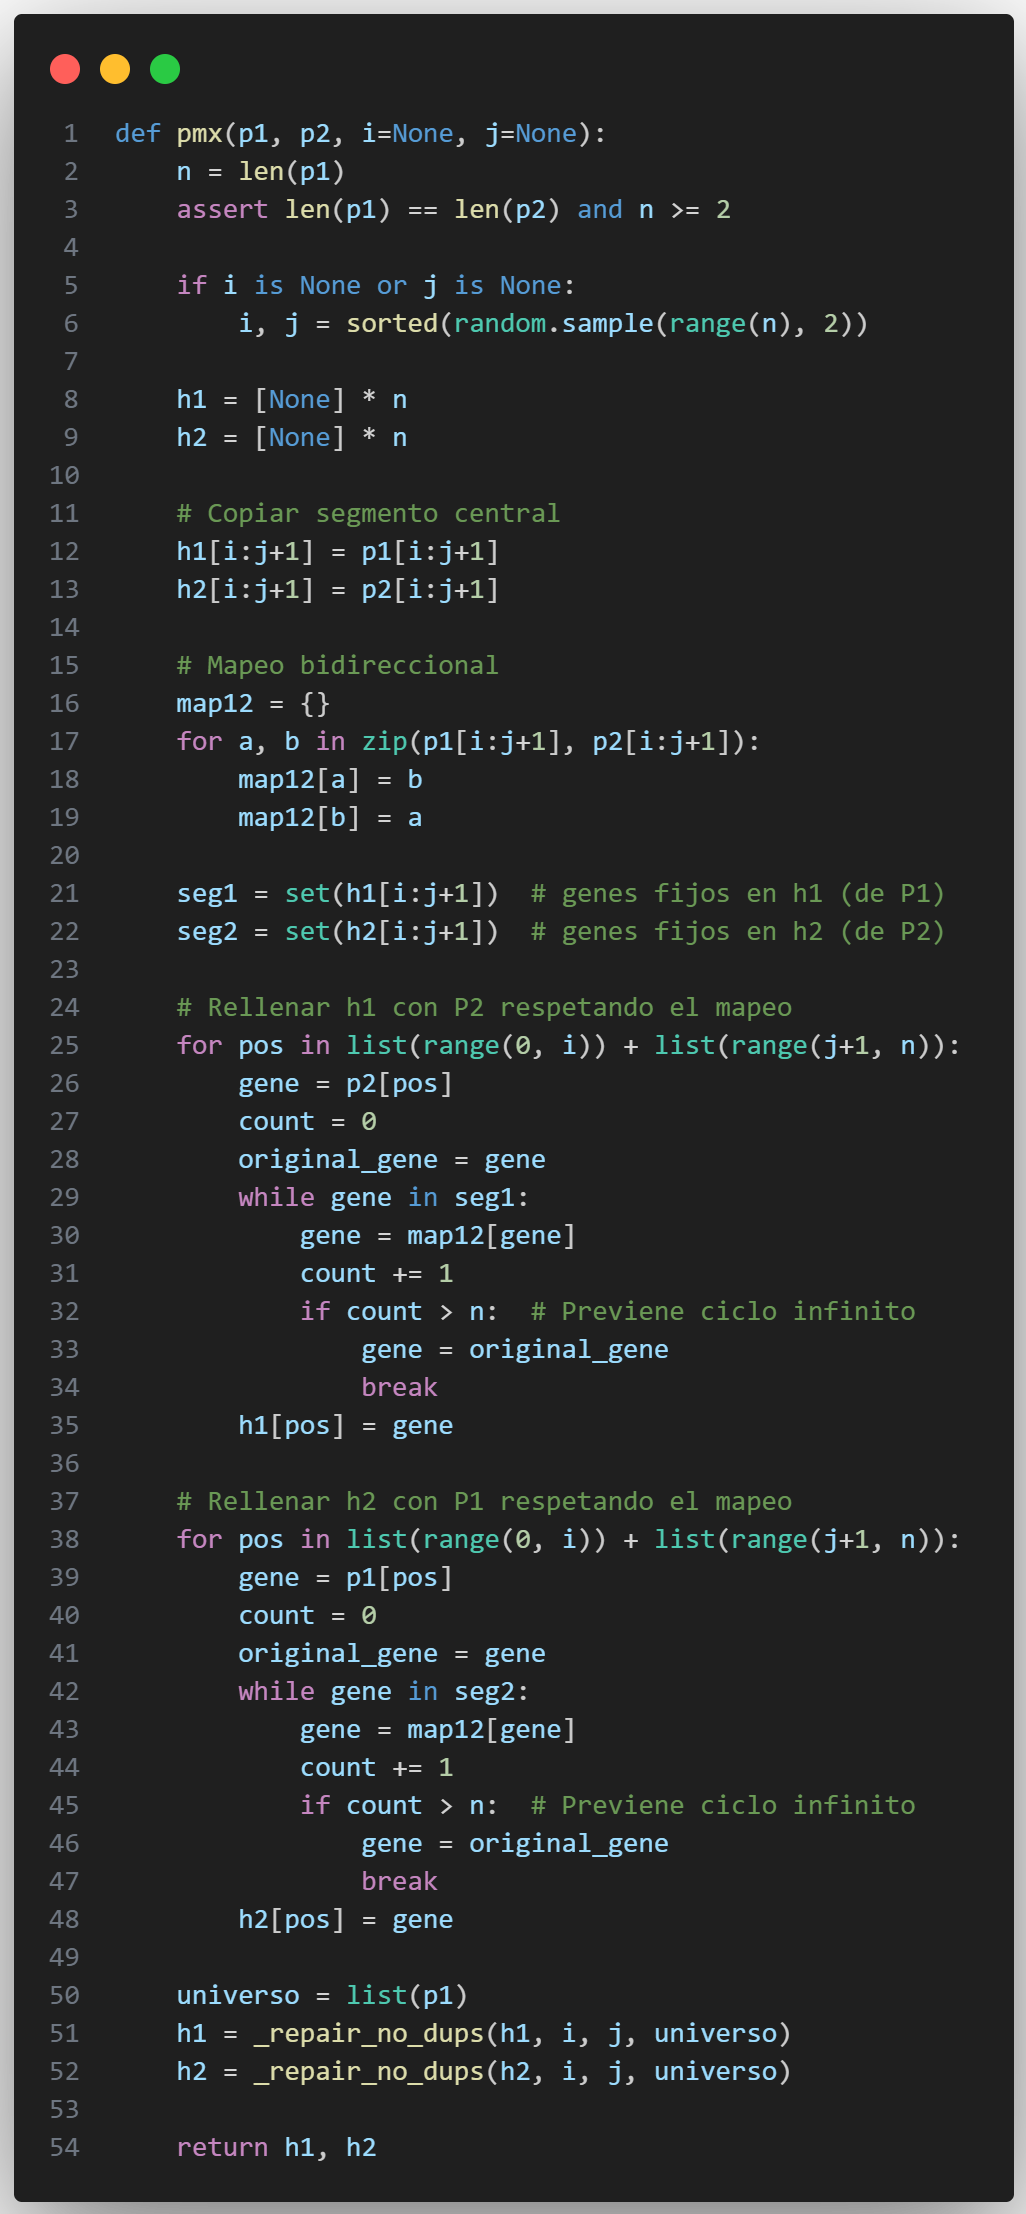
\includegraphics[width=0.45\textwidth]{rsc/img/des/pmx.png}
    \caption{Funcion de cruce PMX}\label{pmx}
\end{figure}

\begin{figure}[H]
    \centering
    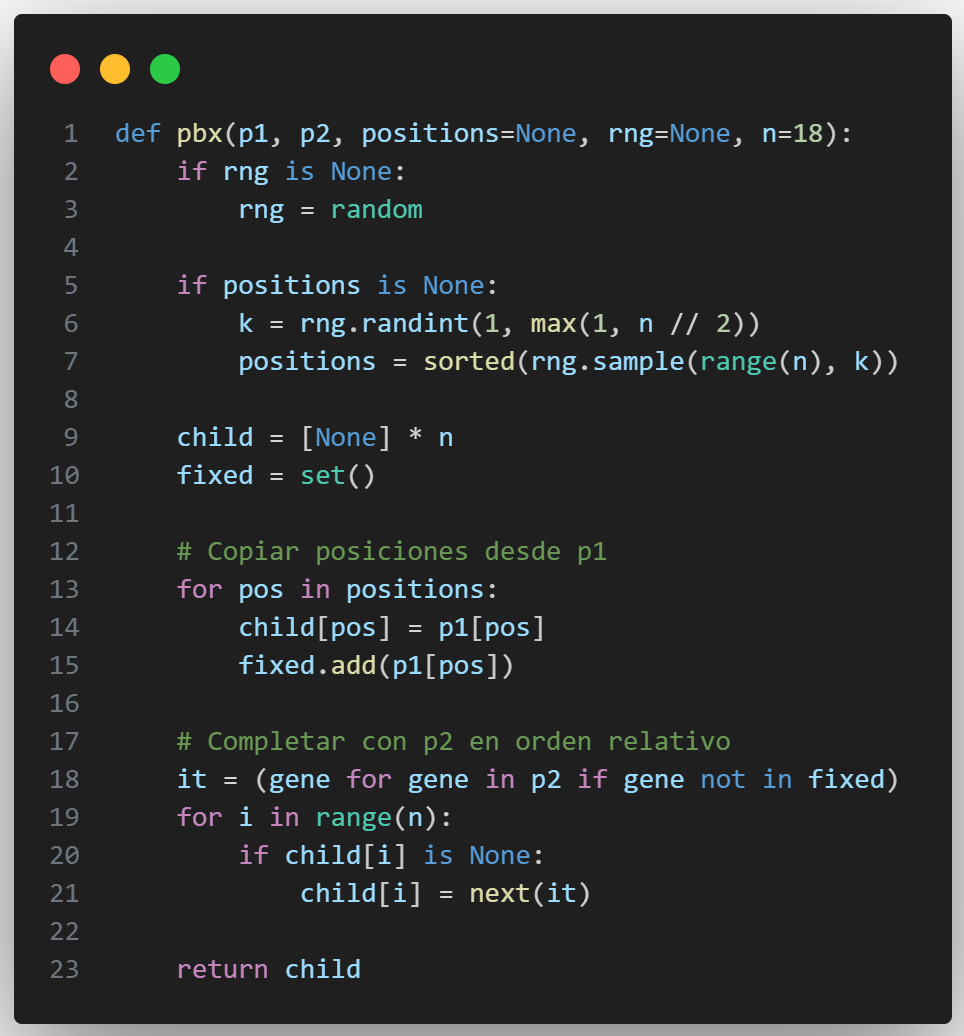
\includegraphics[width=0.65\textwidth]{rsc/img/des/pbx.png}
    \caption{Funcion de cruce PBX}\label{pbx}
\end{figure}

\subsection{Mutación}

Se implementarán dos operadores de mutación: Scramble Mutation y Block Transpose Mutation. La primera selecciona un subconjunto 
aleatorio de ciudades dentro de la ruta y las reordena aleatoriamente, mientras que la segunda intercambia bloques completos de la ruta, 
explorando nuevas configuraciones manteniendo la coherencia de cada bloque.

\begin{figure}[H]
    \centering
    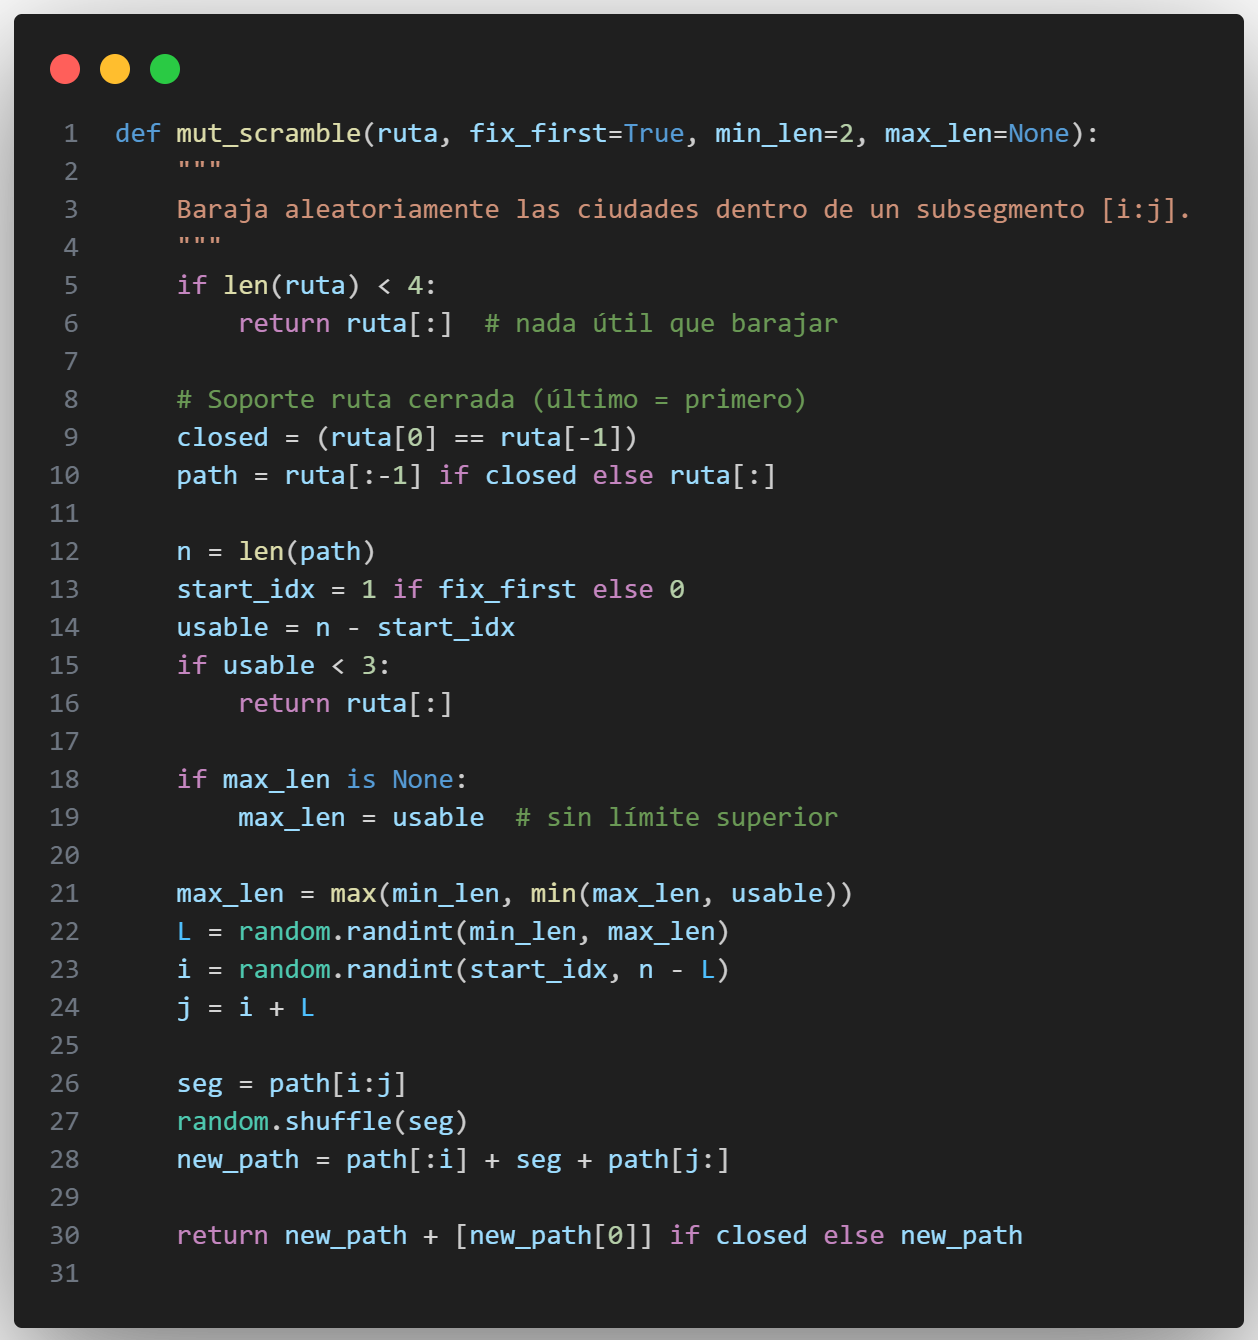
\includegraphics[width=0.5\textwidth]{rsc/img/des/scramble.png}
    \caption{Funcion de mutacion scramble}\label{scramble}
\end{figure}

\begin{figure}[H]
    \centering
    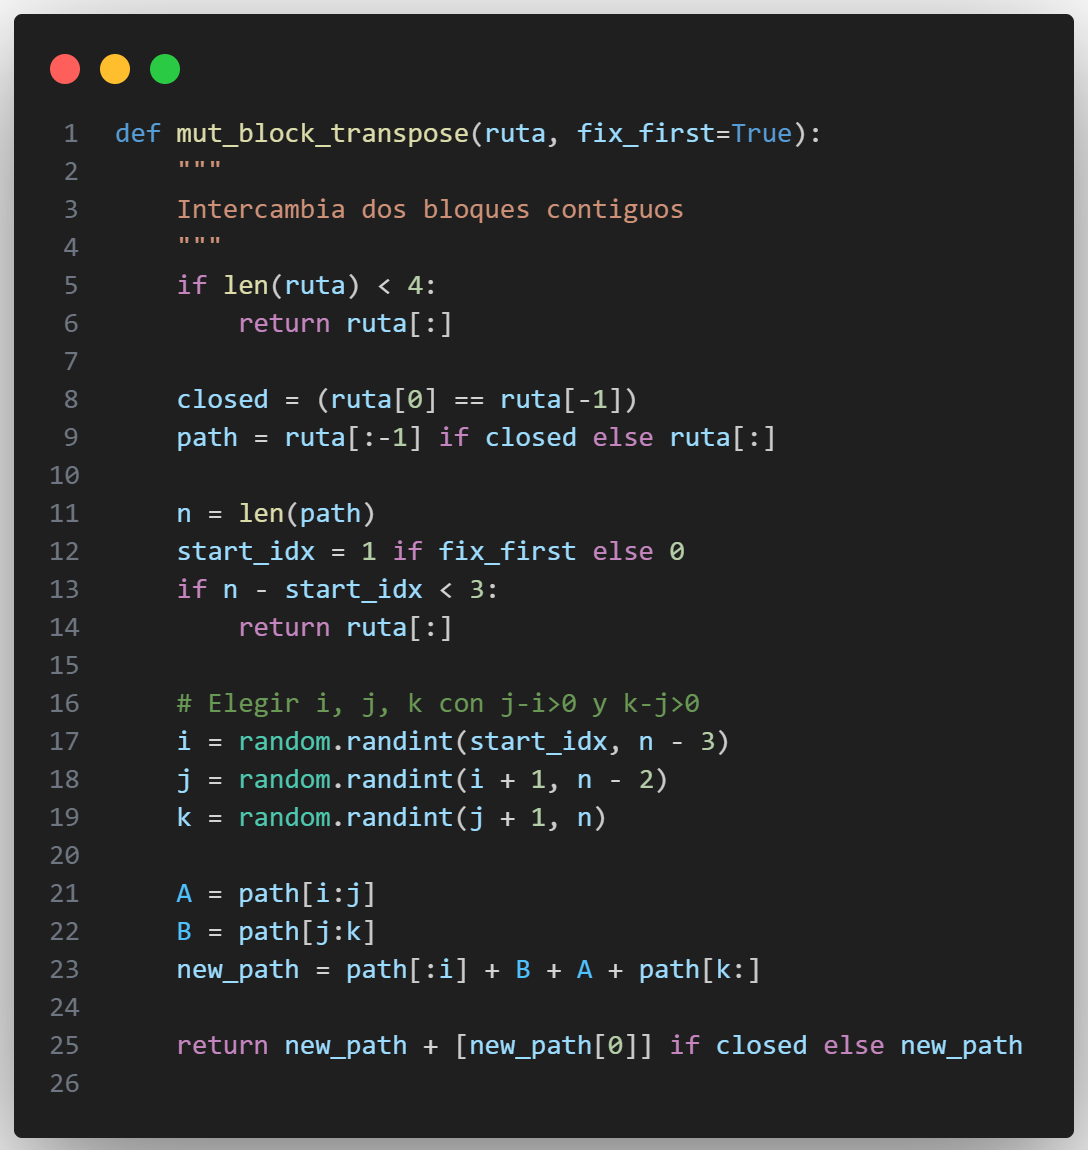
\includegraphics[width=0.5\textwidth]{rsc/img/des/block_transpose.png}
    \caption{Funcion de mutacion block transpose}\label{block_transpose}
\end{figure}

\subsection{Ejecucion del Algoritmo}
Finalmente, se integran todos los componentes anteriores en un algoritmo genético completo que itera a través de generaciones,
aplicando selección, cruce y mutación para evolucionar la población hacia soluciones óptimas, respetando las restricciones de rutas tabú.

\begin{figure}[H]
    \centering
    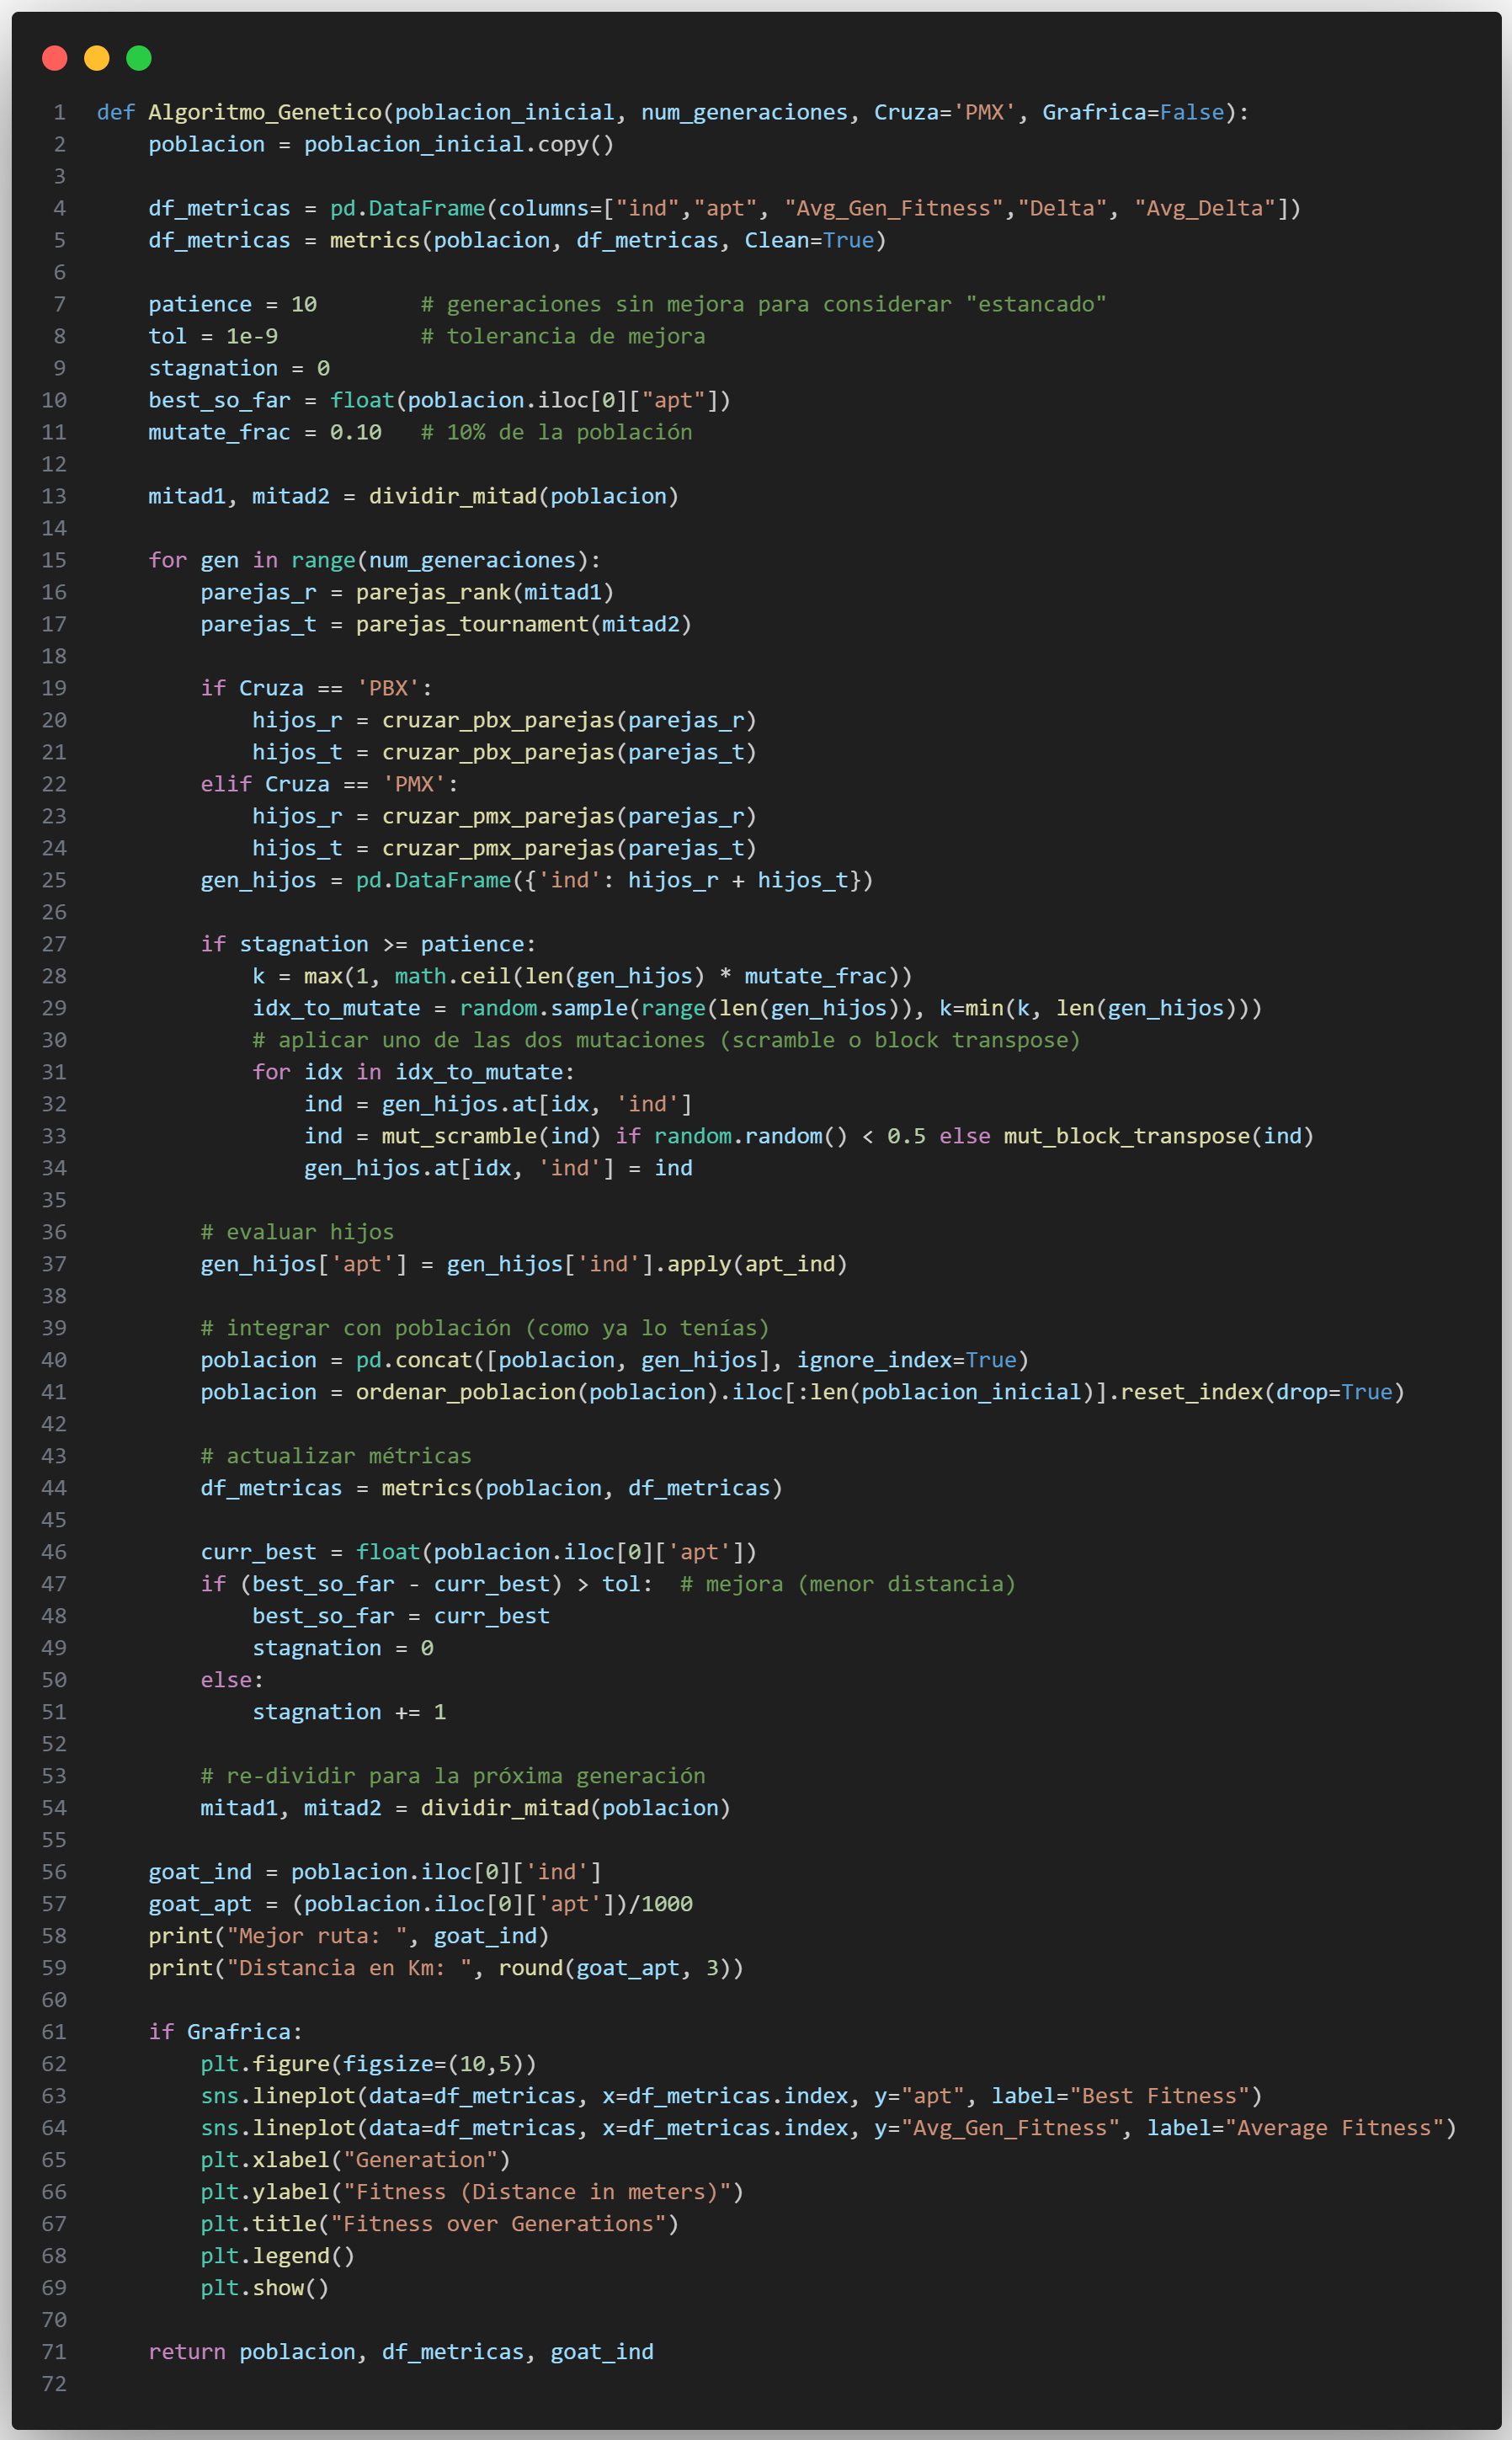
\includegraphics[width=0.65\textwidth]{rsc/img/des/alg_gen.png}
    \caption{Funcion principal del algoritmo genetico}\label{alg_genetico}
\end{figure}

Ejecutaremos este algoritmo con las poblaciones iniciales de tamaños 100, 500 y 1000, observando cómo la diversidad y el tamaño de la población 
afectan la convergencia hacia soluciones óptimas en presencia de restricciones de rutas tabú. Cada ejecución se realizará durante 1000 generaciones 
y se usaran ambos metodos de cruce (PMX y PBX) para comparar su desempeño en este contexto para esto las poblacion se mantienen constantes con cada metodo.

\subsection{Poblacion Inicial: 100} %%%%%%%%%%%%%%%%%%%%%%%%%%%%%%%%%%%%%%%%%%%%%%%%%%%%%%%%%%

\subsubsection{Cruce PMX}\label{100_pmx}

Mejor ruta:  [11, 3, 12, 4, 15, 14, 1, 2, 9, 10, 5, 7, 8, 6, 13, 17, 16, 18]

Distancia en Km:  4677.348

\begin{figure}[H]
    \centering
    
\includegraphics[width=0.75\textwidth]{rsc/img/des/Metrics_100_pmx.png}
    \caption{Evolucion de la mejor aptitud con cruce PMX y poblacion inicial 100}\label{Metrics_100_pmx}
\end{figure}

\begin{figure}[H]
    \centering
    
\includegraphics[width=0.65\textwidth]{rsc/img/des/ruta_100_pmx.png}
    \caption{Mejor ruta encontrada con cruce PMX y poblacion inicial 100}\label{ruta_100_pmx}
\end{figure}

\subsubsection{Cruce PBX}\label{100_pbx}
Mejor ruta:  [9, 10, 5, 11, 2, 1, 14, 15, 4, 3, 12, 13, 6, 7, 8, 17, 16, 18]

Distancia en Km:  4927.898

\begin{figure}[H]
    \centering
    
\includegraphics[width=0.75\textwidth]{rsc/img/des/Metrics_100_pbx.png}
    \caption{Evolucion de la mejor aptitud con cruce PBX y poblacion inicial 100}\label{Metrics_100_pbx}
\end{figure}
\begin{figure}[H]
    \centering
    
\includegraphics[width=0.65\textwidth]{rsc/img/des/ruta_100_pbx.png}
    \caption{Mejor ruta encontrada con cruce PBX y poblacion inicial 100}\label{ruta_100_pbx}
\end{figure}


\subsection{Poblacion Inicial: 500} %%%%%%%%%%%%%%%%%%%%%%%%%%%%%%%%%%%%%%%%%%%%%%%%%%%%%%%%%%

\subsubsection{Cruce PMX}\label{500_pmx}
Mejor ruta:  [12, 3, 4, 15, 14, 18, 16, 17, 13, 6, 8, 7, 5, 11, 10, 9, 2, 1]

Distancia en Km:  4905.76

\begin{figure}[H]
    \centering
    
\includegraphics[width=0.75\textwidth]{rsc/img/des/Metrics_500_pmx.png}
    \caption{Evolucion de la mejor aptitud con cruce PMX y poblacion inicial 500}\label{Metrics_500_pmx}
\end{figure}

\begin{figure}[H]
    \centering
    
\includegraphics[width=0.65\textwidth]{rsc/img/des/ruta_500_pmx.png}
    \caption{Mejor ruta encontrada con cruce PMX y poblacion inicial 500}\label{ruta_500_pmx}
\end{figure}

\subsubsection{Cruce PBX}\label{500_pbx}
Mejor ruta:  [14, 15, 4, 3, 1, 2, 9, 10, 11, 5, 7, 8, 6, 13, 12, 17, 16, 18]

Distancia en Km:  4607.215

\begin{figure}[H]
    \centering
    
\includegraphics[width=0.75\textwidth]{rsc/img/des/Metrics_500_pbx.png}
    \caption{Evolucion de la mejor aptitud con cruce PBX y poblacion inicial 500}\label{Metrics_500_pbx}
\end{figure}

\begin{figure}[H]
    \centering
    
\includegraphics[width=0.65\textwidth]{rsc/img/des/ruta_500_pbx.png}
    \caption{Mejor ruta encontrada con cruce PBX y poblacion inicial 500}\label{ruta_500_pbx}
\end{figure}

\subsection{Poblacion Inicial: 1000} %%%%%%%%%%%%%%%%%%%%%%%%%%%%%%%%%%%%%%%%%%%%%%%%%%%%%%%%%%
\subsubsection{Cruce PMX}\label{1000_pmx}
Mejor ruta:  [7, 8, 6, 13, 12, 4, 15, 14, 1, 2, 9, 10, 5, 11, 3, 17, 16, 18]

Distancia en Km:  4610.896

\begin{figure}[H]
    \centering
    
\includegraphics[width=0.75\textwidth]{rsc/img/des/Metrics_1000_pmx.png}
    \caption{Evolucion de la mejor aptitud con cruce PMX y poblacion inicial 1000}\label{Metrics_1000_pmx}
\end{figure}

\begin{figure}[H]
    \centering
    
\includegraphics[width=0.65\textwidth]{rsc/img/des/ruta_1000_pmx.png}
    \caption{Mejor ruta encontrada con cruce PMX y poblacion inicial 1000}\label{ruta_1000_pmx}
\end{figure}

\subsubsection{Cruce PBX}\label{1000_pbx}\label{MVP}
Mejor ruta:  [1, 2, 9, 10, 11, 5, 7, 8, 6, 13, 12, 3, 4, 15, 14, 17, 16, 18]

Distancia en Km:  4415.911

\begin{figure}[H]
    \centering
    
\includegraphics[width=0.75\textwidth]{rsc/img/des/Metrics_1000_pbx.png}
    \caption{Evolucion de la mejor aptitud con cruce PBX y poblacion inicial 1000}\label{Metrics_1000_pbx}
\end{figure}

\begin{figure}[H]
    \centering
    
\includegraphics[width=0.65\textwidth]{rsc/img/des/ruta_1000_pbx.png}
    \caption{Mejor ruta encontrada con cruce PBX y poblacion inicial 1000}\label{ruta_1000_pbx}
\end{figure}
